\documentclass[twoside,12pt,leqno]{article}
%\documentclass[twoside,12pt,leqno]{report}

\usepackage{amsmath,amssymb,amsfonts,amsthm,mathrsfs,multirow,upgreek}
\usepackage[capposition=bottom]{floatrow} % For Figure Notes
\usepackage{graphicx,pstricks,epstopdf}
\usepackage{url}      % This package helps to typeset urls

%\usepackage{apacite}
%\usepackage{natbib}   % This is a great aid with bibliographies
%\setcitestyle{authoryear,round,semicolon,aysep={},yysep={,},notesep={:}}

\usepackage[title]{appendix}
\renewcommand{\appendixname}{Appendix}

\usepackage[authoryear,comma]{natbib}
\renewcommand{\bibfont}{\small}
\setlength{\bibsep}{0em}

%\usepackage[sc,tiny,center]{titlesec}
\usepackage{titlesec}
\titleformat*{\section}{\sc \center}
\titleformat*{\subsection}{\it \center}
\renewcommand\thesection{\textnormal{{\Roman{section}}}}
\renewcommand{\refname}{Reference}
\usepackage[font={sc,small}]{caption}

\usepackage[%dvipdfmx,%
            bookmarks=true,%
            pdfstartview=FitH,%
            breaklinks=true,%
            colorlinks=true,%
            %allcolors=black,%
            citecolor=blue,
            linkcolor=red,
            pagebackref=true]{hyperref}

\renewcommand{\rmdefault}{ptm}
%\usepackage[lite]{mtpro2}
% use Palatinho-Roman as default font family
%\renewcommand{\rmdefault}{ppl}
\usepackage[scaled=0.88]{helvet}
\makeatletter   % Roman Numbers
\newcommand*{\rom}[1]{\expandafter\@slowromancap\romannumeral #1@}
\makeatother

\newcommand{\E}{\mathbb{E}}
\newcommand{\e}{\mathrm{e}}
\DeclareMathOperator*{\argmax}{argmax}
\renewcommand{\vec}[1]{\ensuremath{\mathbf{#1}}}
\newcommand{\gvec}[1]{{\boldsymbol{#1}}}

\usepackage[hmargin={1.2in,1.2in},vmargin={1.5in,1.5in}]{geometry}
\usepackage{threeparttable,booktabs,multirow} % This allows notes in tables

\usepackage{graphicx}
\usepackage{enumerate}
\usepackage{CJK}
\usepackage[title]{appendix}
\renewcommand{\appendixname}{Appendix}
\newtheorem{result}{Result}
\setlength{\unitlength}{1mm}

\topmargin -1cm        % read Lamport p.163
\oddsidemargin -0.04cm   % read Lamport p.163
\evensidemargin -0.04cm  % same as oddsidemargin but for left-hand pages
\textwidth 16.59cm
\textheight 21.94cm
\renewcommand\baselinestretch{1.15}
\parskip 0.25em
\parindent 1em
\linespread{1}

\newcommand{\code}{\texttt}
\newcommand{\bcode}[1]{\texttt{\blue{#1}}}
\newcommand{\rcode}[1]{\texttt{\red{#1}}}
\newcommand{\rtext}[1]{{\red{#1}}}
\newcommand{\btext}[1]{{\blue{#1}}}

% Set header and footer
%\usepackage{fancyhdr}
%\pagestyle{fancy}
%\fancyhead{}
%\fancyhead[LE,RO]{\thepage}
%\cfoot{}
%\renewcommand{\headrulewidth}{0pt}

%\pdfoptionpdfminorversion 6

\begin{document}

\title{\large{THE LETTER TO THE DATA EDITOR}}
\date{}
\maketitle

\vspace{-1.75cm}

\begin{flushleft}
Dear AEA Data Editor,
\end{flushleft}

This letter summarizes our response to the second report from you on our revision to the repository (OPENICPSR-112005). We sincerely appreciate the careful investigation of the replication team into our programs again.

In the report, the team reported possible discrepancies between Figures 2 and E.1 with their underlying variable value from the code. However, we have doubled checked on this, and found no discrepancies between the figures and the code output after executing the programs (\bcode{Empirical\_AEJ.R} and \bcode{Empirical\_Appendix.R}) on our computer. We suspect that the reason this happened is because in this revision, we have removed the National Economic Census data of China as requested in the previous revision. As a result, Section 3 of \bcode{Empirical\_AEJ.R} and Section 5 of \bcode{Empirical\_Appendix.R} cannot be run in bulk appropriately without the Chinese data. %The discrepancies identified by the team may be some intermediate results when the programs terminate due to missing data.

To address this issue, we have uploaded a new program \bcode{Empirical\_Public\_Data.R} that reproduces the empirical results relying only on the published Statistics of U.S. Businesses data. The file reproduces the U.S. firm distributions, which are exactly the same as those in the paper. Figures \ref{fig:fig2left} to \ref{fig:fige1br} (appended to the end of this report) provide direct comparison of the reproduced results to each panel in Figure 2 and E.1. We have also revised the README file by introducing a new Section \rom{1}.D (alongside with Tables 1 and 2) explaining which results can be reproduced readily with the data published in the repository and how to do so.

%If the team would like to verify the whole process manually, it should be done as follows. This process essentially produces file \bcode{Data\_Rev\_2.R}. We will use only the left panel of Figure 2 (pooled polluting) as an example. The rest cases are virtually the same procedure applied to different data.
%\begin{enumerate}
%    \item
%    Open file \bcode{Empirical\_AEJ.R}. Execute lines 26 to 33, to load necessary \code{R} packages.
%    \item
%    Execute lines 215 to 218 to load the U.S. firm size distribution raw data.
%    \item
%    Execute lines 233 to 258, to select the polluting industries and compute the average firm size in each size bin.
%    \item
%    Comment out lines 263 to 265 in the \code{for} loop, as they are computing the total employment within each size bin for China. Once they are commented out, execute lines 260 to 270, which will store the density of each bin in vector \bcode{distus}. In this case, it equals to $[0.056, 0.111, 0.189, 0.644]$, which is consistent with the blue bar in Figure 2 (left panel).
%    \item
%    Slightly modify the syntax to plot the vector would generate the figures in this report.
%\end{enumerate}

\newpage
\begin{figure}[h]
    \begin{center}
    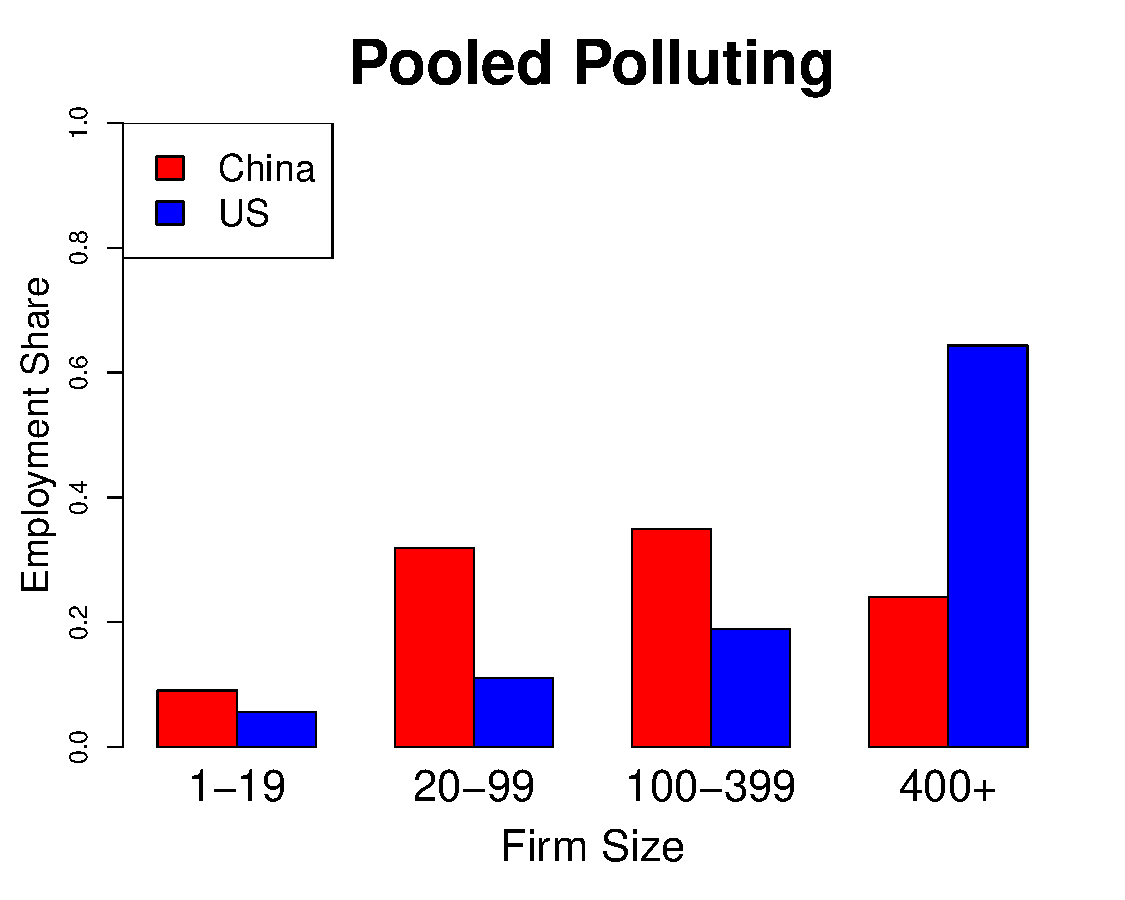
\includegraphics[width=0.45\textwidth]{./Figures/Figure2_Left.pdf}
    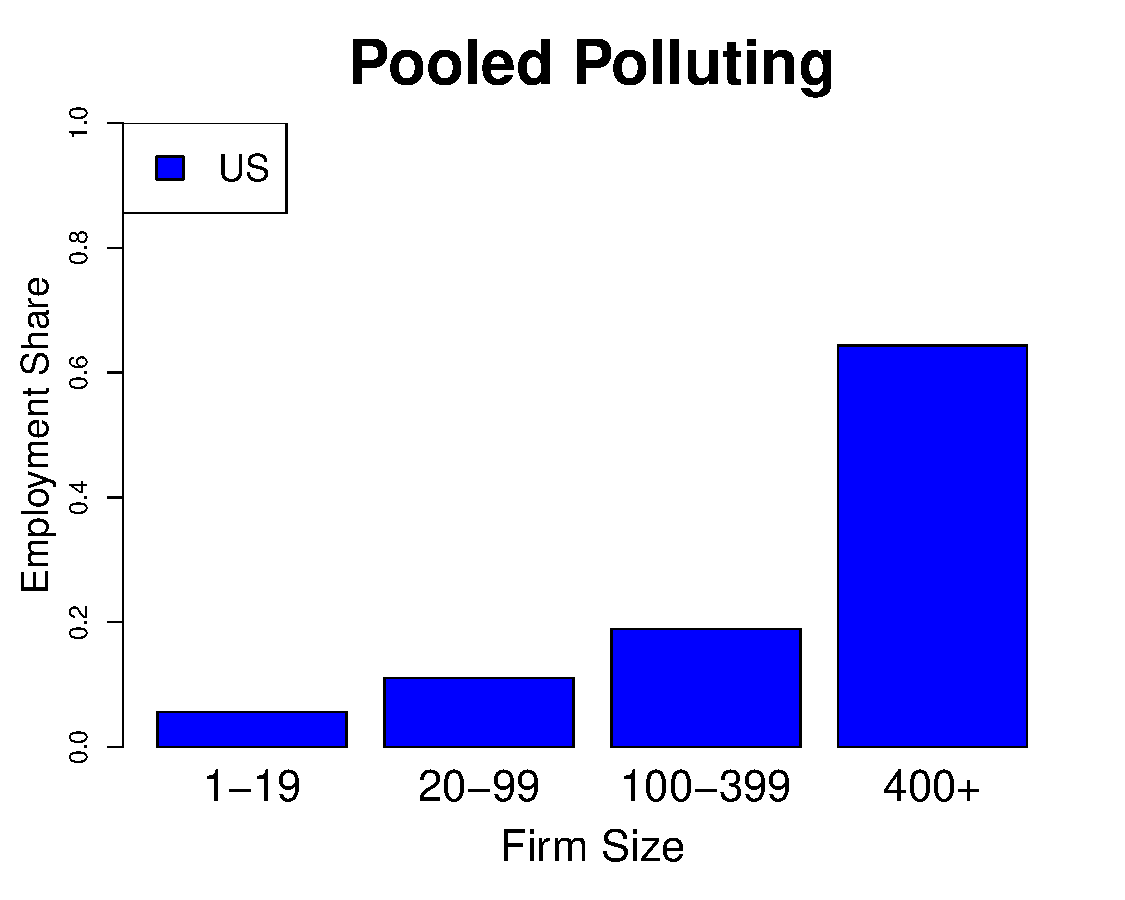
\includegraphics[width=0.45\textwidth]{./Figures/Figure2_US_Left.pdf}
    \caption{Main Text Figure 2 Left Panel}
    \label{fig:fig2left}
    \end{center}
\end{figure}

\begin{figure}[h]
    \begin{center}
    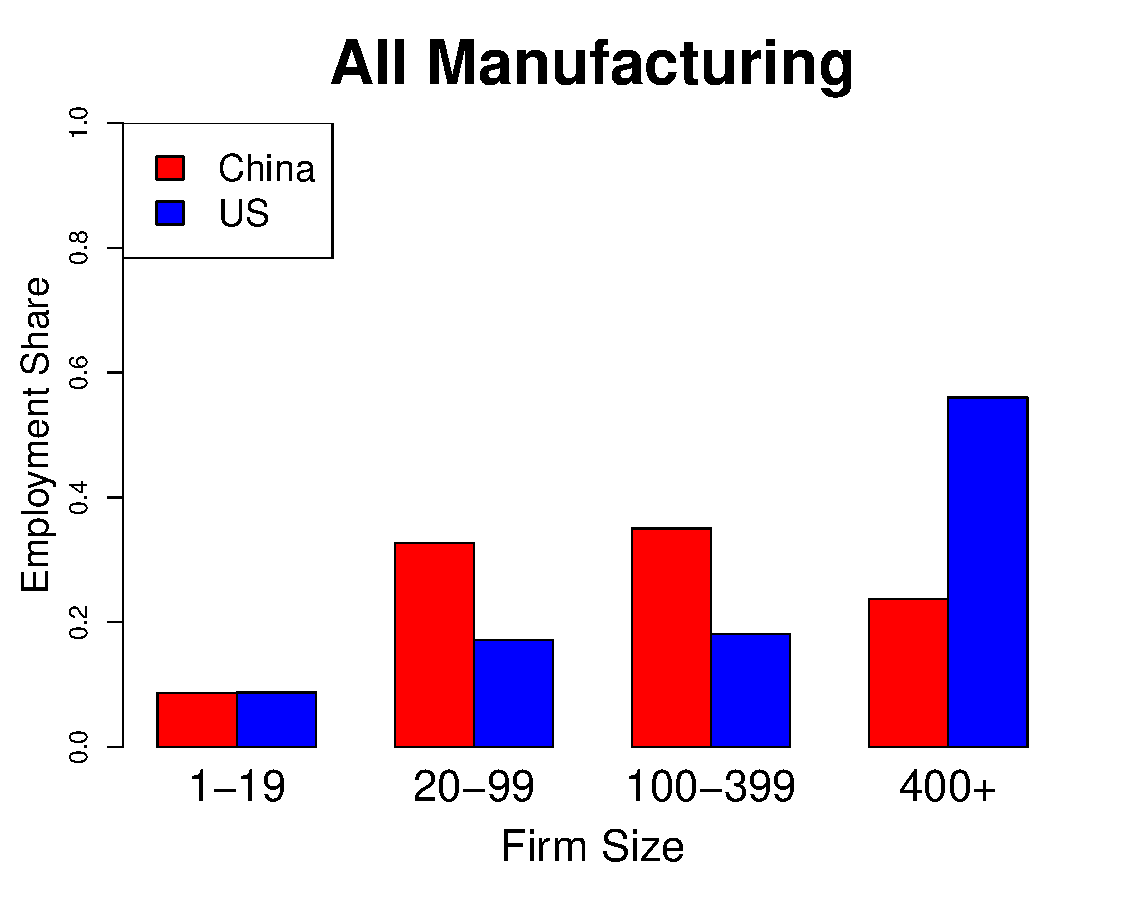
\includegraphics[width=0.45\textwidth]{./Figures/Figure2_Right.pdf}
    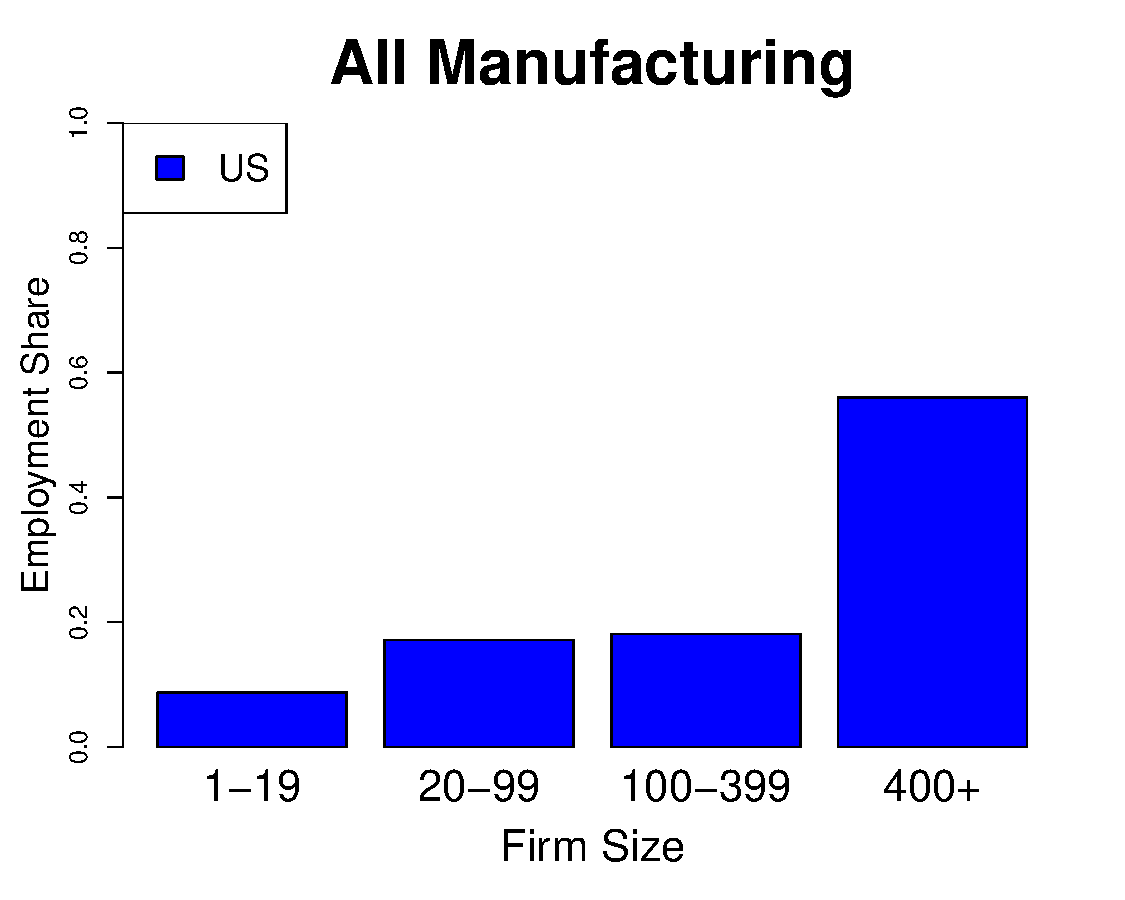
\includegraphics[width=0.45\textwidth]{./Figures/Figure2_US_Right.pdf}
    \caption{Main Text Figure 2 Right Panel}
    \end{center}
\end{figure}

\begin{figure}[h]
    \begin{center}
    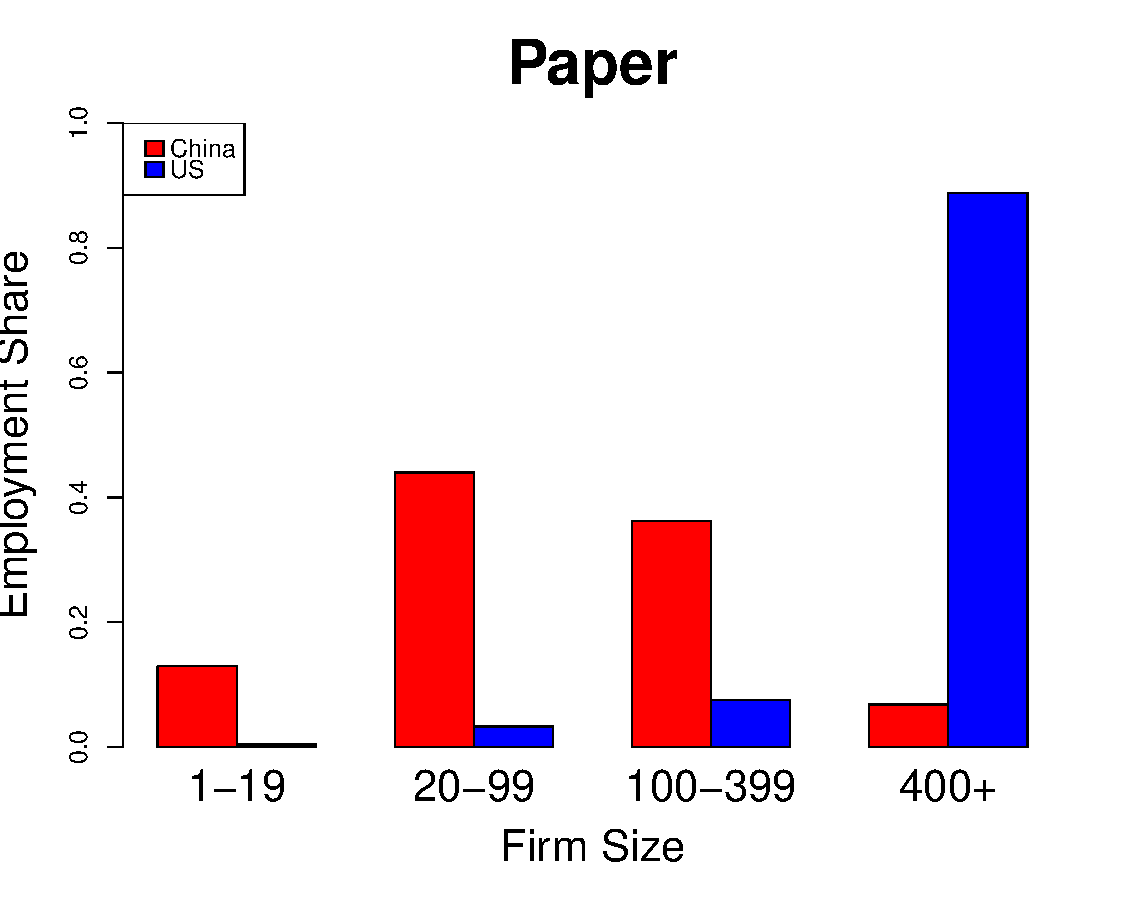
\includegraphics[width=0.45\textwidth]{./Figures/FigureE1_TopLeft.pdf}
    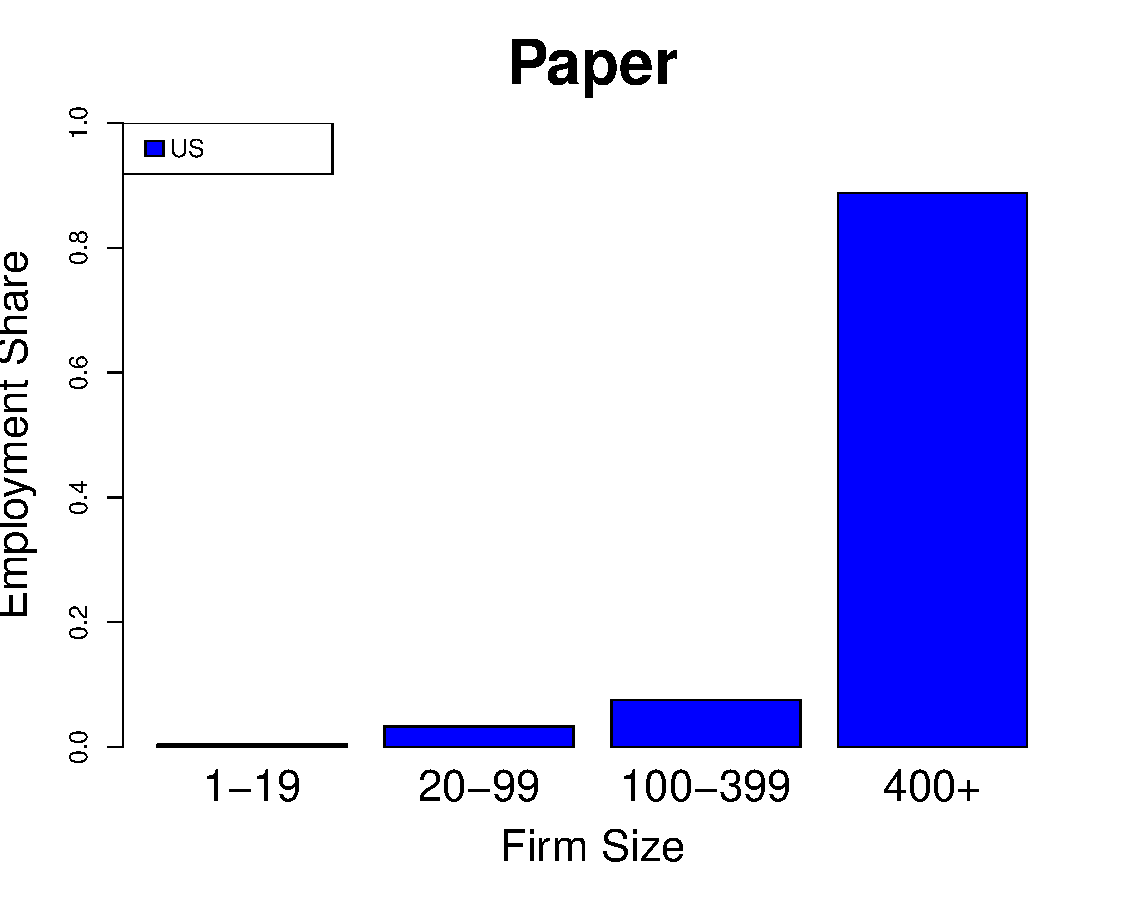
\includegraphics[width=0.45\textwidth]{./Figures/FigureE1_US_TopLeft.pdf}
    \caption{Appendix Figure E.1 Top Left Panel}
    \end{center}
\end{figure}

\begin{figure}[h]
    \begin{center}
    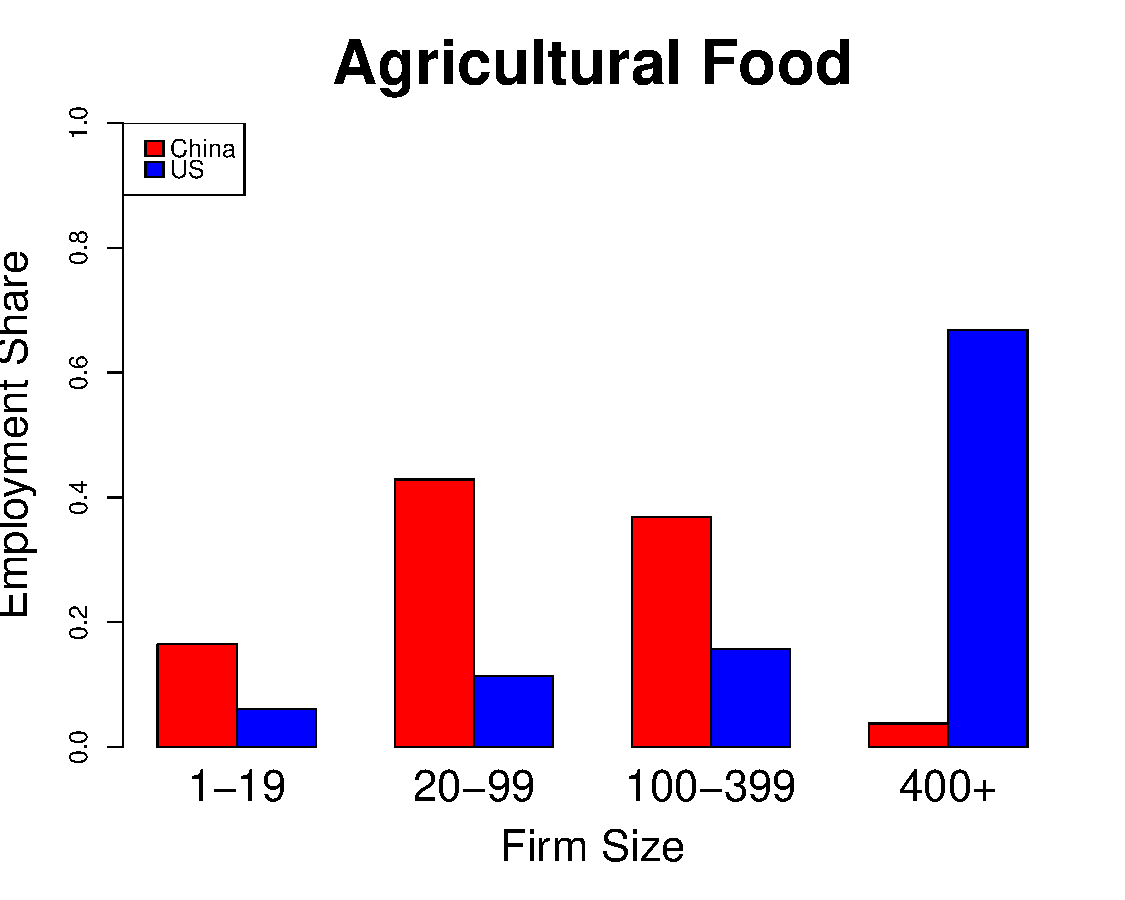
\includegraphics[width=0.45\textwidth]{./Figures/FigureE1_TopRight.pdf}
    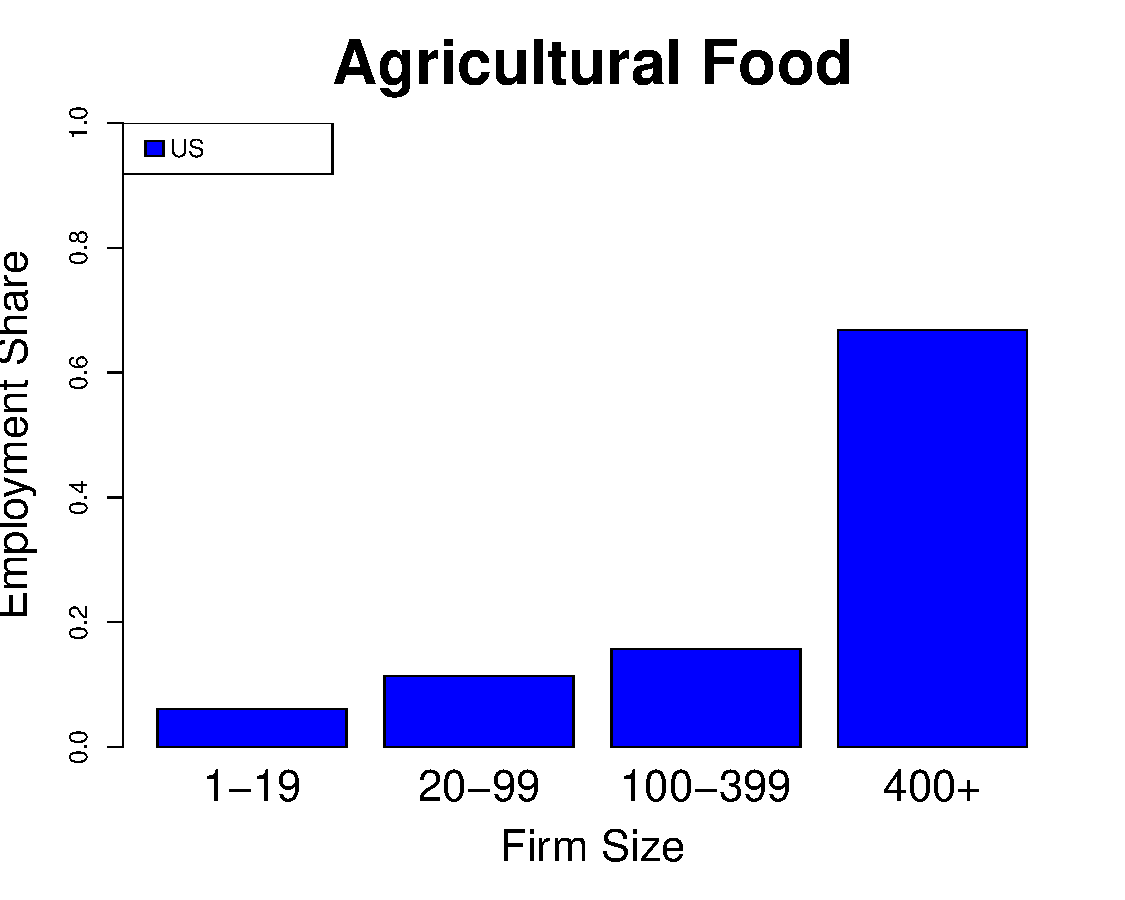
\includegraphics[width=0.45\textwidth]{./Figures/FigureE1_US_TopRight.pdf}
    \caption{Appendix Figure E.1 Top Right Panel}
    \end{center}
\end{figure}

\begin{figure}[h]
    \begin{center}
    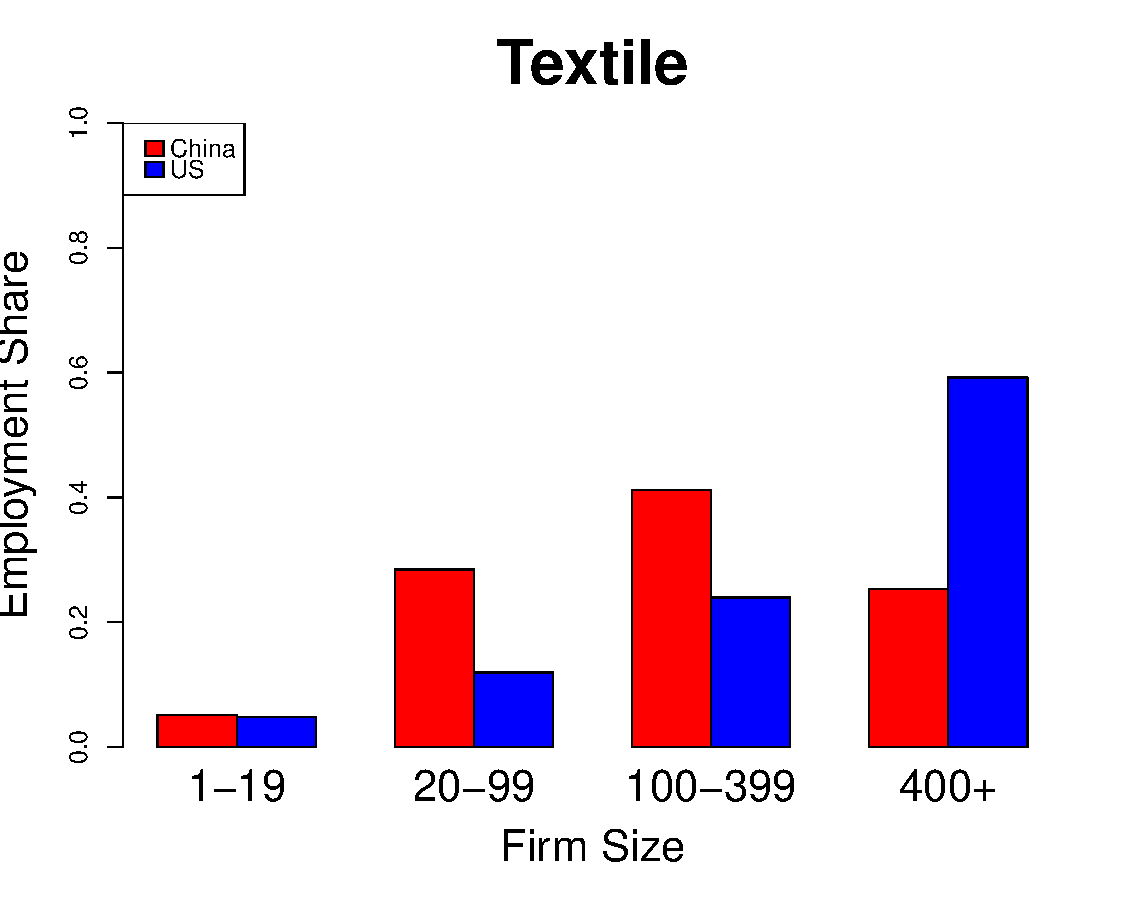
\includegraphics[width=0.45\textwidth]{./Figures/FigureE1_MidLeft.pdf}
    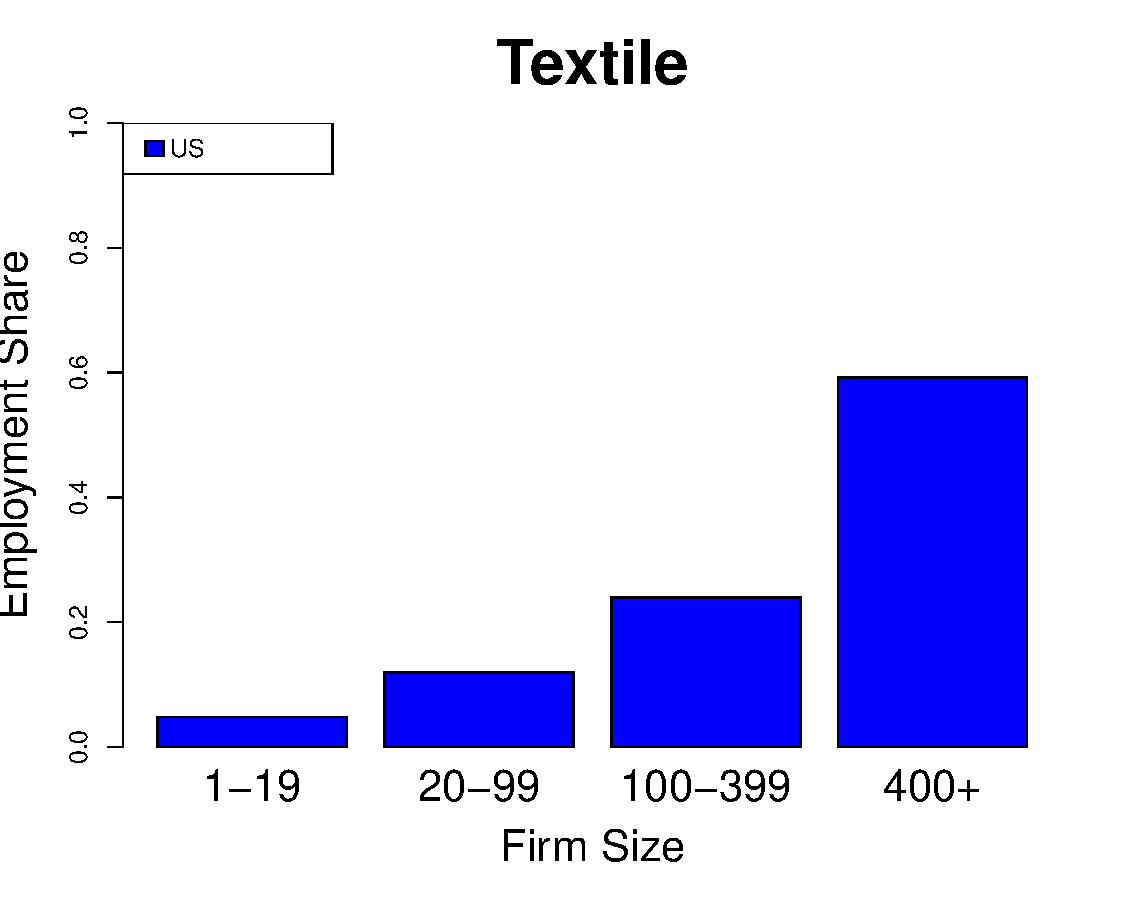
\includegraphics[width=0.45\textwidth]{./Figures/FigureE1_US_MidLeft.pdf}
    \caption{Appendix Figure E.1 Mid Left Panel}
    \end{center}
\end{figure}

\begin{figure}[h]
    \begin{center}
    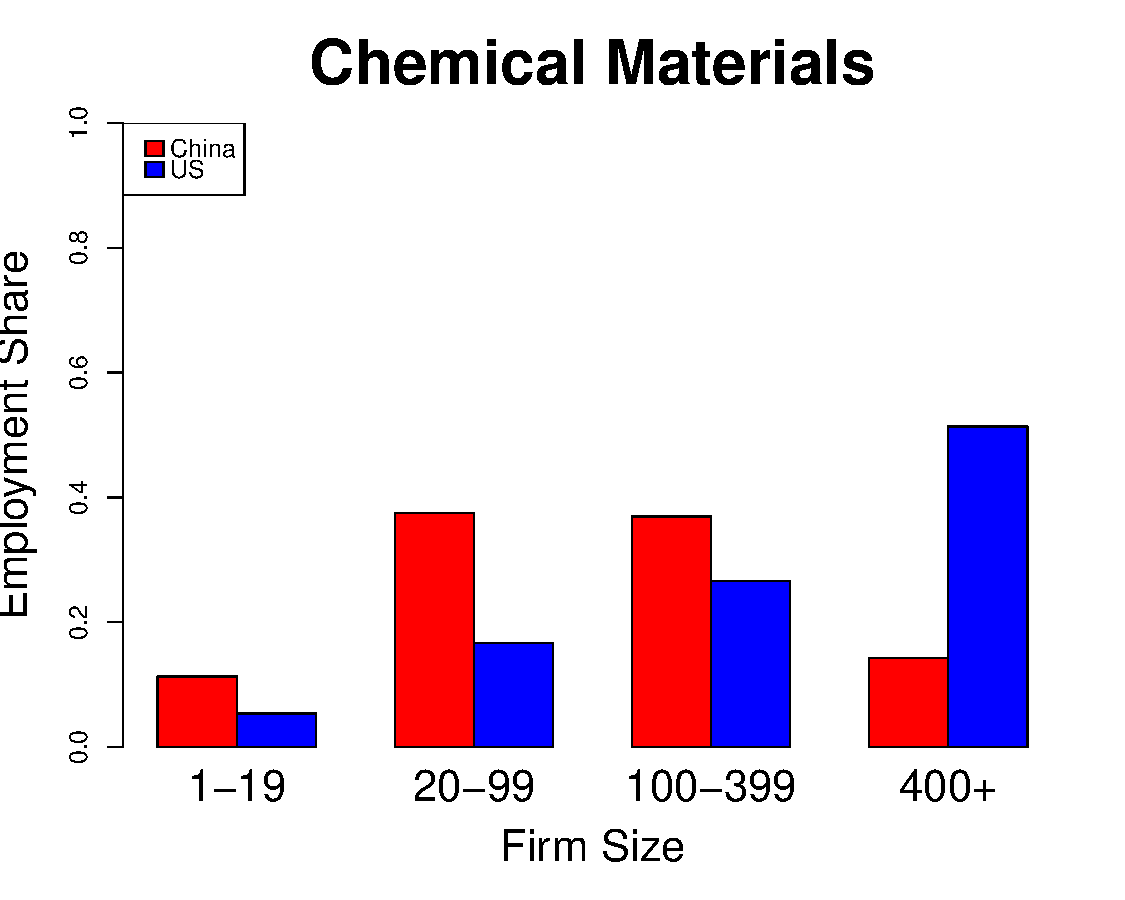
\includegraphics[width=0.45\textwidth]{./Figures/FigureE1_MidRight.pdf}
    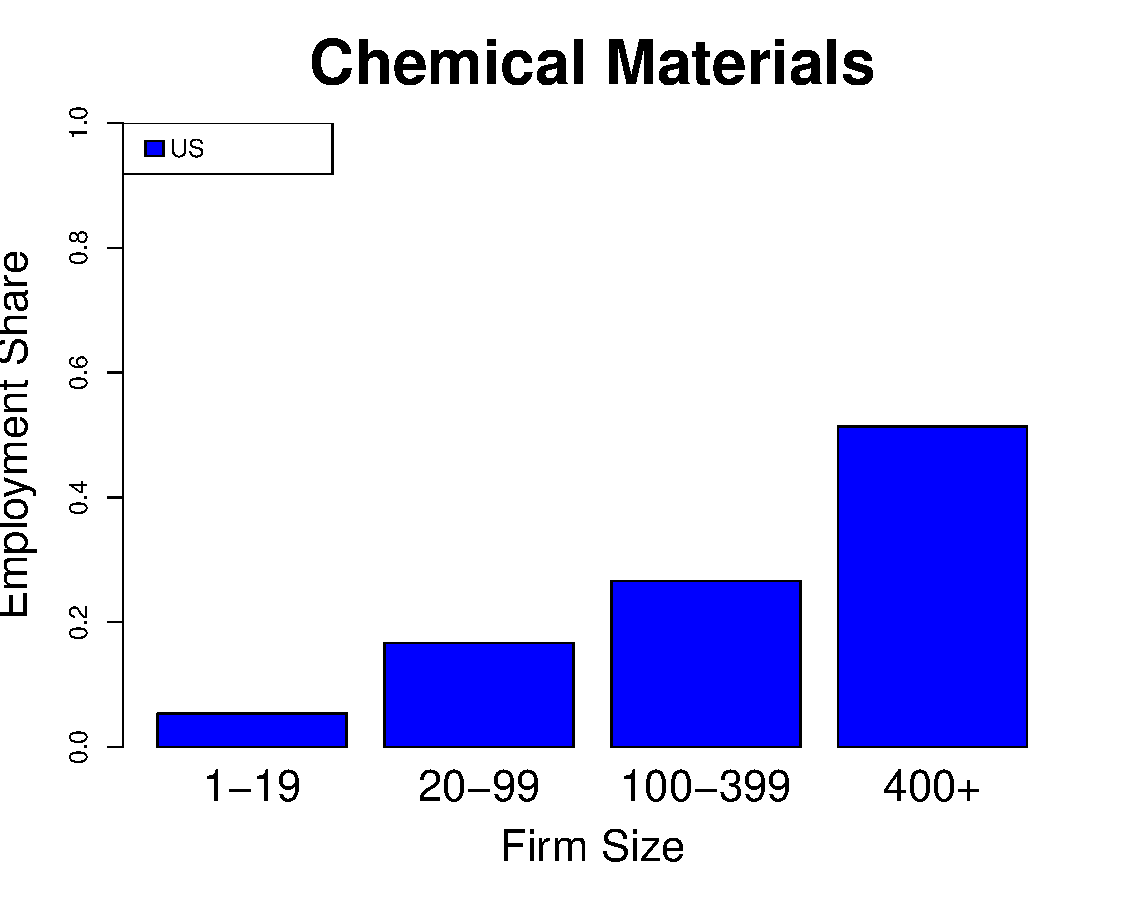
\includegraphics[width=0.45\textwidth]{./Figures/FigureE1_US_MidRight.pdf}
    \caption{Appendix Figure E.1 Mid Right Panel}
    \end{center}
\end{figure}

\begin{figure}[h]
    \begin{center}
    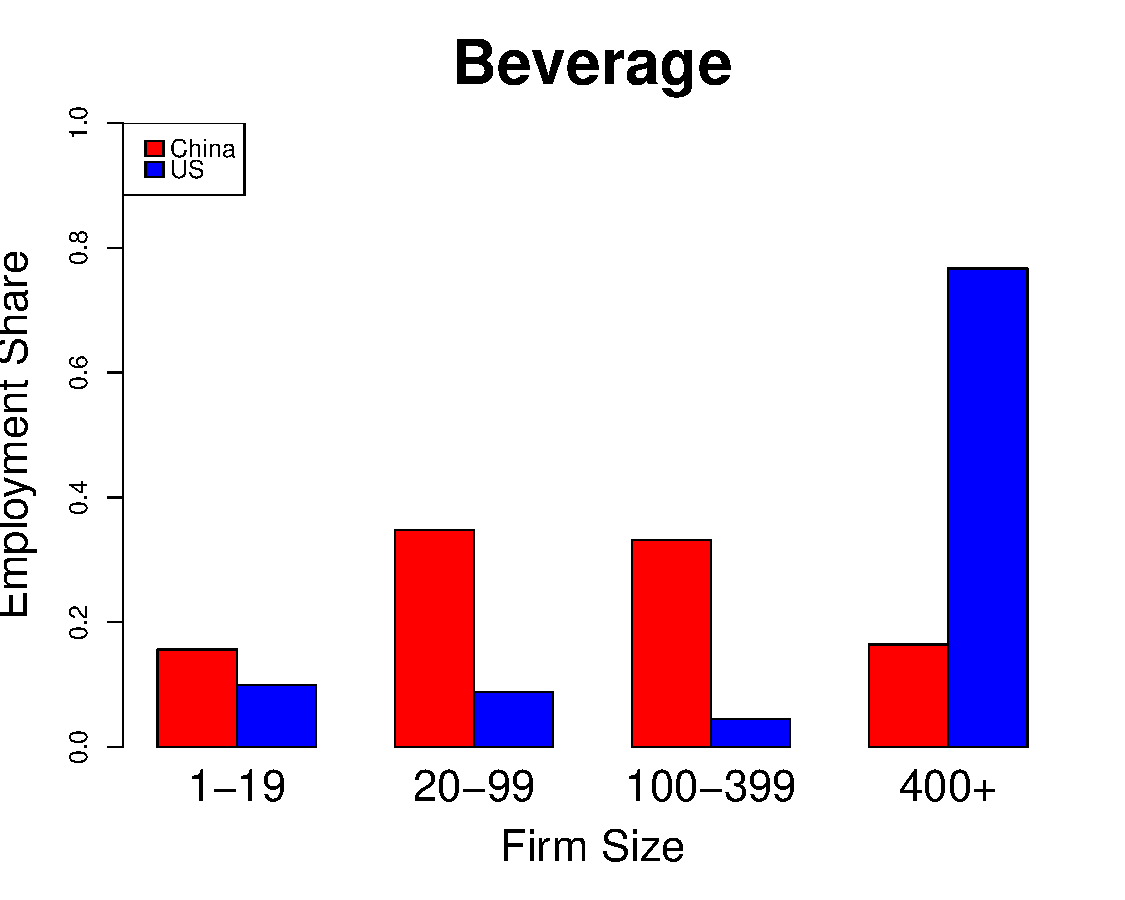
\includegraphics[width=0.45\textwidth]{./Figures/FigureE1_BotLeft.pdf}
    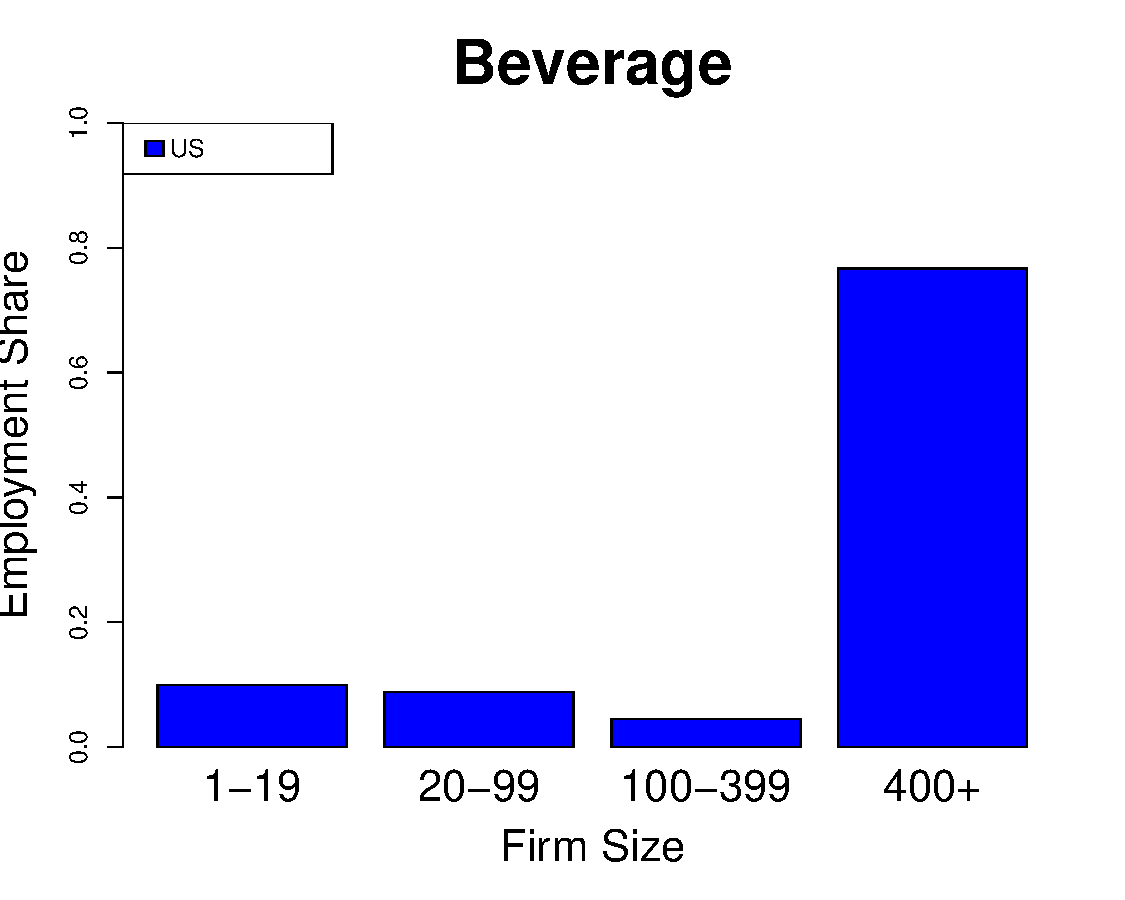
\includegraphics[width=0.45\textwidth]{./Figures/FigureE1_US_BotLeft.pdf}
    \caption{Appendix Figure E.1 Bottom Left Panel}
    \label{fig:fige1br}
    \end{center}
\end{figure}

\end{document}
